\section{Testszenarien} %
\label{sec:Testszenarien}
In diesem Abschnitt werden die Testszenarien beschrieben, wie die einzelnen Hardwarekomponenten FPGA und ESP32, wie auch die Verbindungen unter den Komponenten getestet wurden.

\subsection{FPGA Decodierung und SPI Test}
\label{sub:FPGADecSPITest}
Um zu Verifizieren ob die Decodierung des Manchester-Signal und die Ausgabe der Daten per SPI korrekt funktionieren, wurde mittels Matlab und der Software "'ArbExpress"' ein vom MVB aufgenommenes Signal so aufbereitet, dass dies mit dem Signalgenerator \textit{Tektronix AFG 3102} abgespielt werden konnte. Mit dem Tektronix ist es möglich über die beiden Outputs A \& B ein differentielles Signal auszugeben. Somit wurde das Signal (siehe Abbildung \ref{fig:ReineDaten}) welches zur Bestimmung der Busauslastung aufgenommen wurde, mit dem Tektronix abgespielt. Das Signal wurde anschliessend über den RS485-Transceiver auf den FPGA geführt. Der Ausgang des FPGA mit den ausgewerteten Daten wurde über SPI auf das \textit{Picoscope 2207B} geführt. Mit der Software "'PicoScope 7"' konnten die ausgegebenen Daten gelesen und analysiert werden. Es wurden verschieden grosse Telegramme aufbereitet und zur Überprüfung mit dem Signalgenerator ausgegeben. In einer ersten Phase wurde der Test ohne die Implementierung des 64-Bit-Puffers durchgeführt. Da der ESP32 mehr Zeit zur Verarbeitung der Daten benötigte, wurde, wie in Kapitel \ref{fpga:spi} beschrieben, eine Pufferung der Daten implementiert, bevor diese per SPI übertragen werden. Folglich wurde auch das FPGA mit dem implementierten Puffer gestestet\\
In Abbildung \ref{fig:TestszenarioFPGA} ist der Testaufbau des FPGA zu sehen.

\begin{figure}[H]
    \centering
    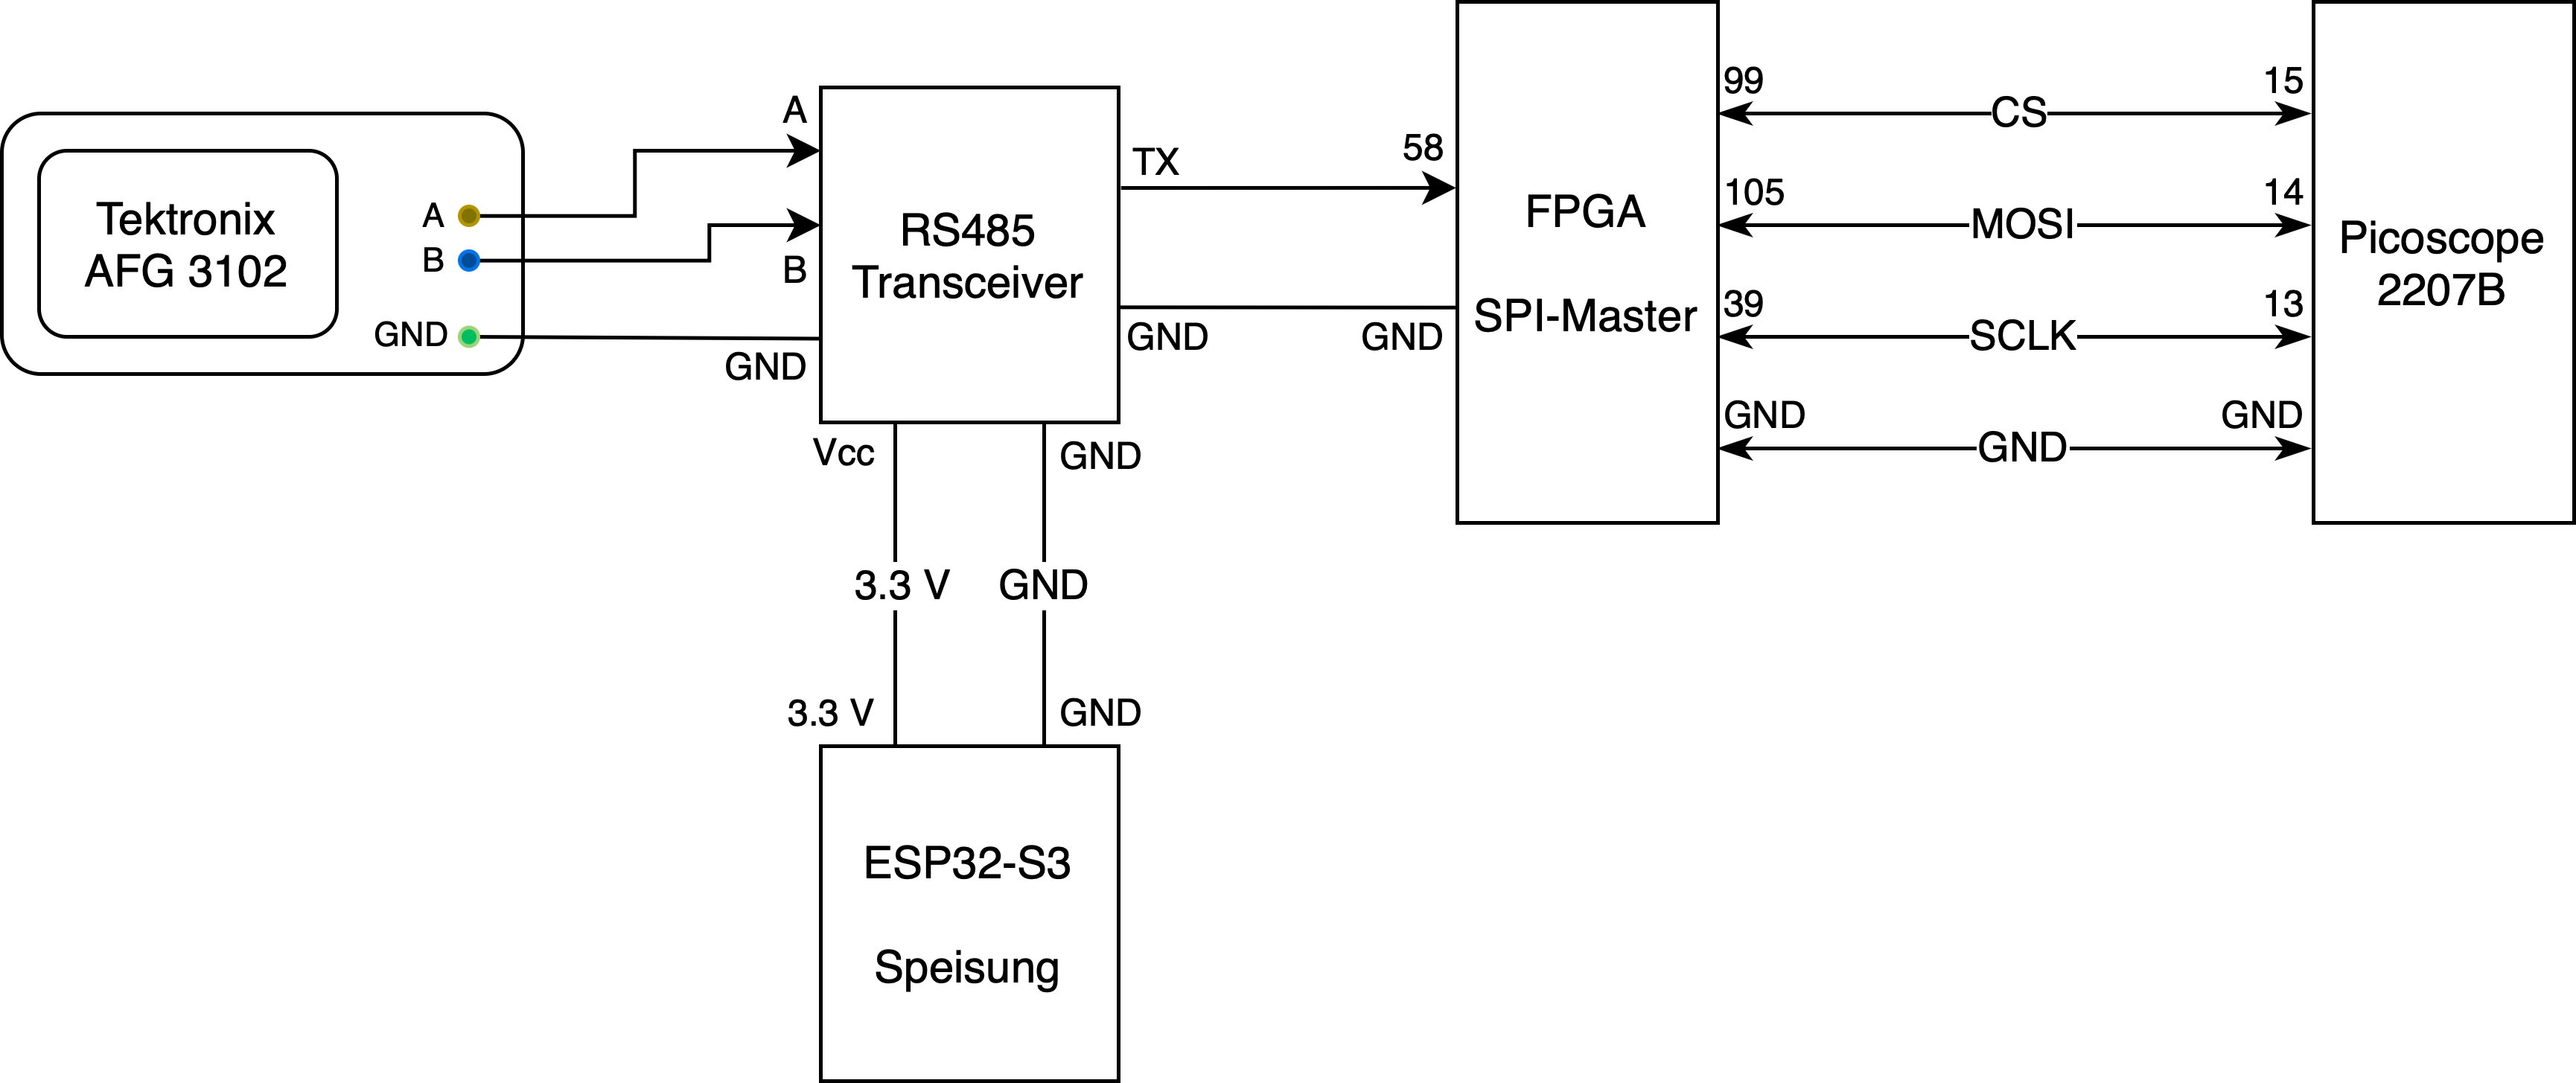
\includegraphics[width=0.9\linewidth]{Figures/Chap3/Testszenarien/Testszenario_FPGA.png}
    \caption{Testaufbau zum Testen der Manchester Decodierung auf dem FPGA}
    \label{fig:TestszenarioFPGA}
\end{figure}

Für den Test wurden folgende Einstellungen am Tektronix vorgenommen:\\
\\
\textbf{Frequenz:}\hspace{1.87cm} \textbf{4.295 KHz} (Um eine Datenrate von \textbf{1.5 Mbits/s} zu erreichen)\\
\textbf{Spannungsbereich:}\hspace{0.25cm} \textbf{0 V - 5 V}\\
\\
Der Tektronix wurde auf Burst eingestellt, wodurch das Telegramm immer wieder nach der eingestellten Zeit abgespielt wird.
Dabei wurde der Test mit \textbf{100 ms} und \textbf{1 ms} Zeit zwischen dem abgespielten Signal durchgeführt. Bei 1 ms wird die Auslastung, wie diese auf dem MVB statt findet,
simuliert.\\
\\
Es wird erwartet dass die Daten, wie diese in der Tabelle \ref{tab:frame_data} zu sehen sind, übertragen werden. Diese Daten sollen mit in der Software \textit{Picoscope 7} ersichtlich sein.

\begin{table}[h!]
    \centering
    \begin{tabular}{r||l||l}
        \toprule
        \textbf{Frame Type} & \textbf{Data}  & \textbf{Payload} \\ 
        \midrule
        Master Frame 1 & 0xC715’569A’6555’99A6 & 0x1B'40'AD \\
        Slave Frame 1  & 0xA8E3’5565’9A65’AAAA’AAAA’6A66 & 0x04'B4'FF'FF'75 \\
        \midrule
        Master Frame 2 & 0xC715’5595’6955’A9AA & 0x08'60'EF \\
        Slave Frame 2  & 0xA8E3’5555’5555’AAAA & 0x00'00'FF\\
        \midrule
        Master Frame 3 & 0xC715’5699’5A55’6AAA & 0x1A'30'7F \\
        Slave Frame 3  & 0xA8E3’5565’A996’AAAA’AAAA’A569 & 0x04'E9'FF'FF'C6 \\
        \midrule
        Master Frame 4 & 0xC715’9656’5655’6AA9 & 0x91'10'7E\\
        \bottomrule
    \end{tabular}
    \caption{Master and Slave Frame Data}
    \label{tab:frame_data}
\end{table}




\subsection{ESP32 SPI und Statemachine Test}
\label{sub:ESPSPIundFSMTest}

Für die Verifikation der Firmware auf dem ESP32-S3 wurde ein zweites Gerät, welches als SPI-Master den FPGA simulieren soll, verwendet. Die Hardware, welche als SPI Master verwendet wurde, war ein ESP32. Dies aus dem Grund, weil bereits Erfahrungen mit dem ESP32 vorhanden waren und das Aufsetzen des Gerätes, sowie das Ausgeben von Daten über die SPI schnell realisiert werden konnten. In Abbildung \ref{fig:TestszenarioESP32} ist der schematische Aufbau zu sehen. Es wurden die Verbindungen für die SPI-Leitungen und GND verbunden. Auf einem Laptop wurde die Open-Source-Software Bluetility, ein Tool für Bluetooth Low Energy, verwendet. Mit dieser Anwendung können Geräte gescannt, deren Dienste und Eigenschaften durchsucht, sowie Werte gelesen, geschrieben und abonniert werden. Gemäss Kapitel \ref{sub:BluetoothGATT} wurden die Daten in der Charakteristik mit der roten Zahl 1 empfangen. Zusätzlich wird die Reaktionszeit beim Empfangen der SPI-Daten gemessen. Dies wird durch das Vergleichen der Chip Select-Leitung und der Handshakeleitung \textcolor{red}{berechnet.?} 

\begin{figure}[H]
    \centering
    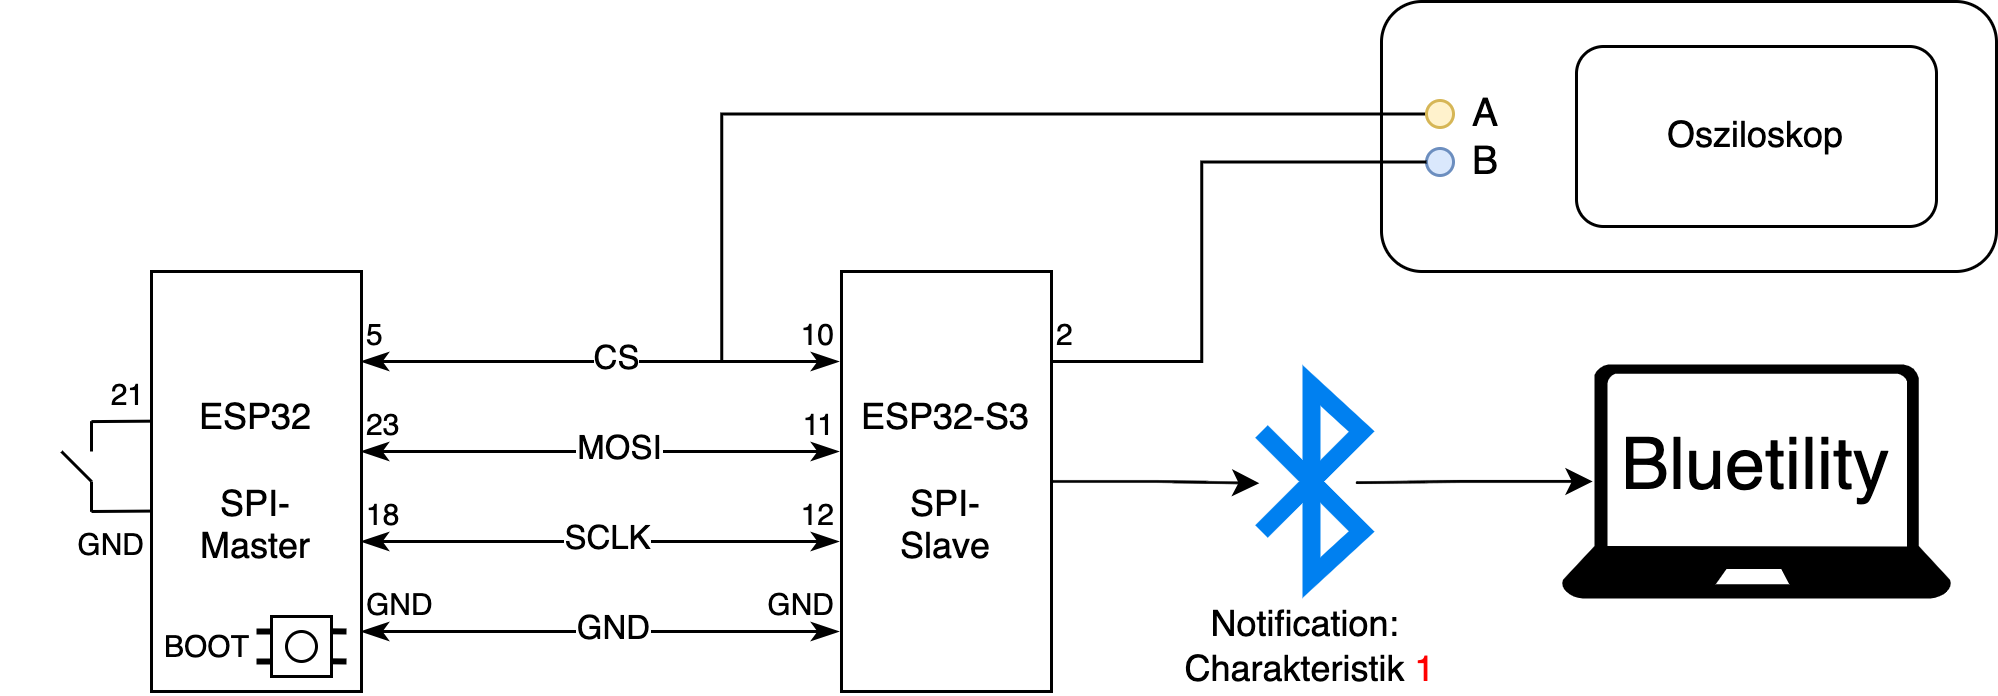
\includegraphics[width=0.9\linewidth]{Figures/Chap3/Testszenarien/Testszenario_ESP32.png}
    \caption{Testaufbau zum Testen der Manchester Decodierung auf dem ESP32-S3}
    \label{fig:TestszenarioESP32}
\end{figure}

Der SPI-Master konnte zwei unterschiedliche Telegramme schicken. Es kann entweder das kürzeste oder das längste Telegramm geschickt werden. Die Auswahl ist von Pin 21 (siehe Abbildung \ref{fig:TestszenarioESP32}) abhängig. Wird dieser Pin zu Ground gezogen, wird das lange Telegramm geschickt. Bleibt der Kontakt offen, wird das kurze Telegramm gesendet. Das Senden eines Paketes wird durch Drücken des Boot-Knopfes ausgelöst. Dies zieht den Pin 0 zu Ground , was im Programm ausgewertet werden kann. 

Der Inhalt, der in Tabelle \ref{tab:TestDataESP32} zu sehen ist, sind die Nutzdatenbits, welche vom SPI Master geschickt werden. Der SPI-Master schickt die Daten wie der FPGA Manchester encodiert in 64 Bit-Päckchen, also jeweils 32 Bit Nutzdatenbits. Bei den Slave Daten wurde absichtlich ein lesbarer ASCII String für die Dummy Daten verwendet, da diese in Bluetility direkt ersichtlich ist.

\begin{table}[H]
    \centering
    \begin{tabular}{r||l|l}
         & Kurz & Lang\\ \hline
        FCode & 9 (0x9) & 12 (0xC)\\ \hline
        Addresse & 0x101 & 0x0D8\\ \hline
        Master Check & 0xF0 & 0x21\\ \hline
        Slave Data & NH & Hello World 01234567890123456789\\ \hline
        Slave Check & 0x53 & 0x5A 0x98 0x70 0x5d\\ 
    \end{tabular}
    \caption{Testdaten für Testszenario ESP32}
    \label{tab:TestDataESP32}
\end{table}

Folgende Zeiten werden mit dem Oszilloskop gemessen und die Werte entsprechend in den Resultaten dargestellt. Diese werden in der Diskusion aufgegriffen:
\begin{itemize}
    \item Reaktionszeit: Die Zeit zwischen positiver Flanke der Chip-Select-Leitung (Kanal A) und der negativen Flanke der Handshake-Leitung (Kanal B)
    \item Back-to-Receive-Zeit (BTR-Zeit): Die Zeit zwischen positiver Flanke der Chip-Select-Leitung und der positiven Flanke der Handshake-Leitung.
\end{itemize}

\subsection{Verbindungstest ESP32 zu FPGA}
\label{subsec:VerbindugstestESP32FPGA}

Um zu testen ob die Decodierung des Manchestersignal bis hin zur Übertragung via Bluetooth korrekt funktioniert, wurde ein Testaufbau des ganzen Sniffers realisiert. Für den Aufbau wurden die verschiedenen Komponenten des Sniffers wie in Abbildung \ref{fig:TestszenarioSniffer} zu sehen ist, verbunden.

\begin{figure}[H]
    \centering
    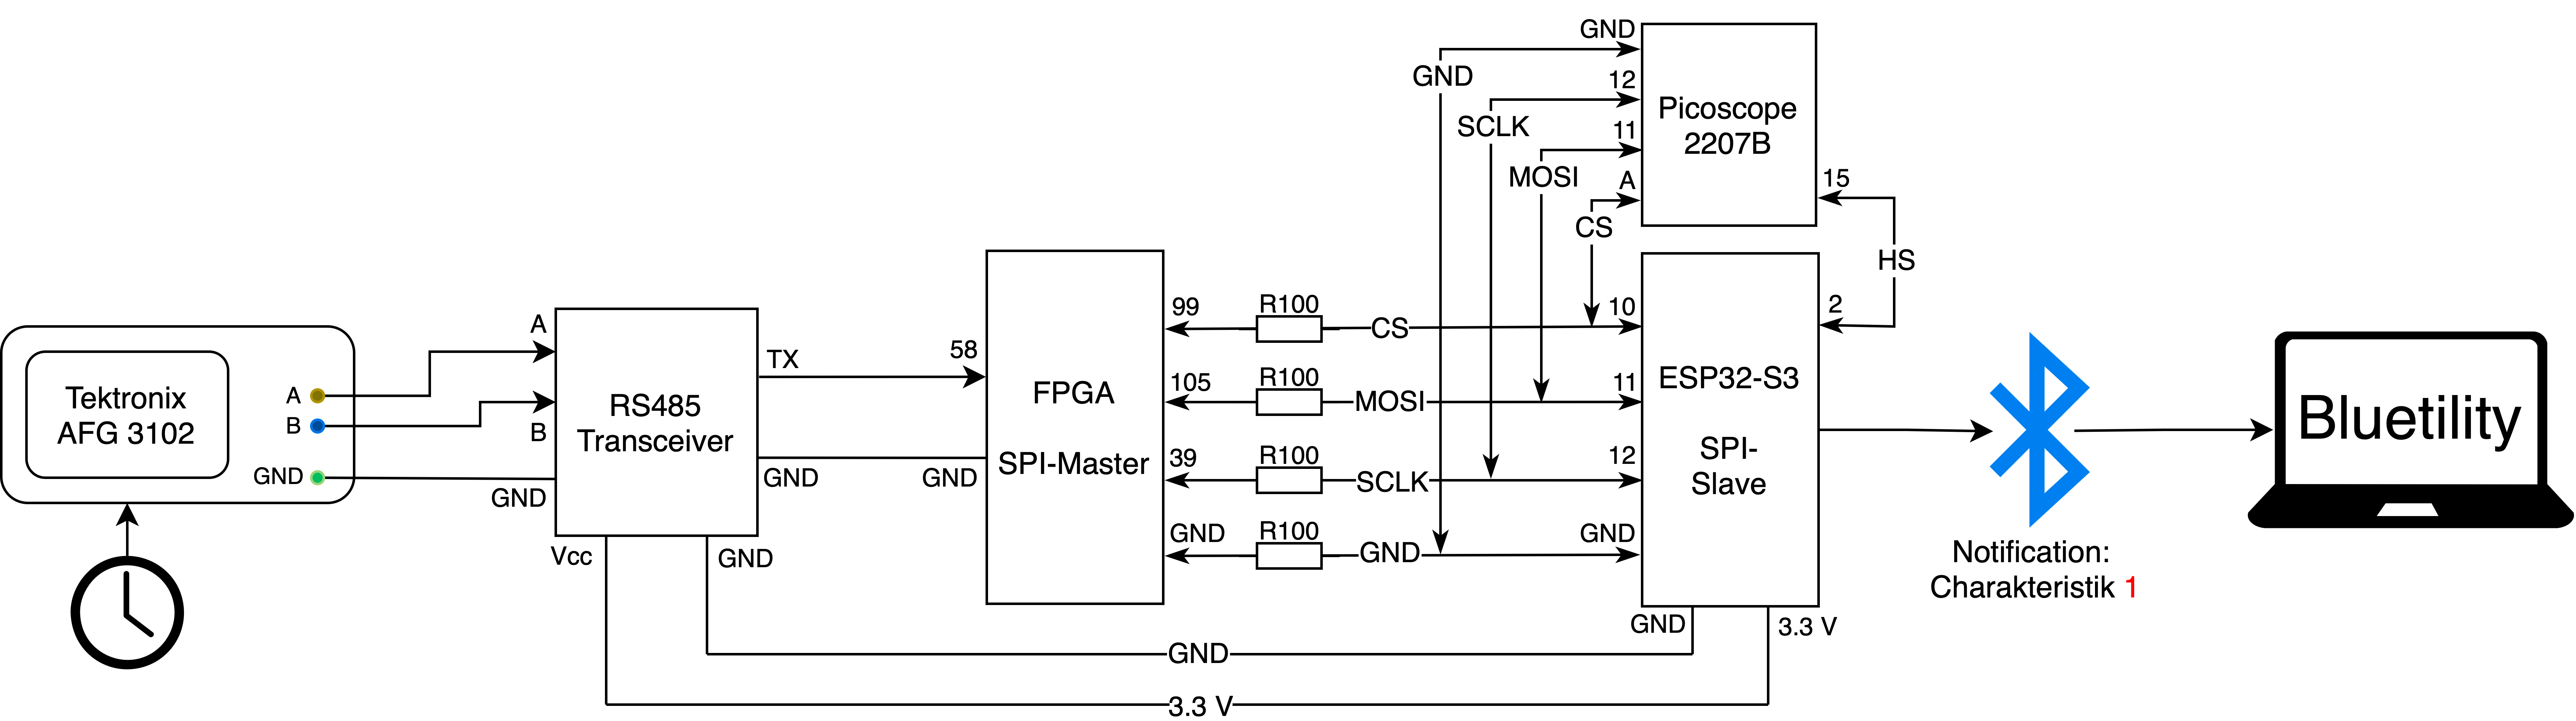
\includegraphics[width=1\linewidth]{Figures/Chap3/Testszenarien/Testszenario_Sniffer.png}
    \caption{Testaufbau zum Testen des Sniffer}
    \label{fig:TestszenarioSniffer}
\end{figure}


Als Signalquelle wurde, wie in Kapitel \ref{sub:FPGADecSPITest} beschrieben, der Signalgenerator \textit{Tektronix AFG 3102} mit den gleichen Einstellungen verwendet. Das Triggerintervall wird auf 3 Sekunden eingestellt.\\
In diesem Testaufbau wurden die gleichen Daten, wie diese in der Tabelle \ref{tab:frame_data} in der Spalte \textit{Data} zu sehen sind, übertragen. Als Ausgabe über Bluetooth wird der Payload, welcher ebenfalls in der Tabelle \ref{tab:frame_data} in der Spalte \textit{Payload} aufgelistet ist, erwartet.


\subsection{Stresstest FPGA zu ESP32}
\label{sub:MethStesstest}

Bei einem höheren Triggerintervall ist die händische Auswertung mit Picoscope und Bluetility nicht mehr genau genug. Differenzen in der Übertragung können erkennt werden, jedoch sind diese schnell wieder aus dem Bufferbereich verschwunden und die Daten verloren.

Aus diesem Grund wurde eine andere Methode verwendet, um den Stresstest des FPGA, der Verbindung zum ESP und dessen Übertragung über Bluetooth zu testen. Der Testaufbau ist wie in Abbildung \ref{fig:TestszenarioSniffer} aufgebaut, jedoch wurde das Picoscope entfernt und die Übertragung über Bluetooth angepasst. 

Mit ChatGPT wurde ein Python Script geschrieben, welches auf die Charakteristik subscribed, die empfangenen Daten in einem CSV File abspeichert und anschliessend mit einem weiteren Script eine Auswertung vornimmt. Der Code ist in Anhang \ref{app:File62} (logger.py) und \ref{app:File61} (analyse.py) zu finden. In Abbildung \ref{fig:TestszStresstest} ist eine schematische Abbildung davon zu sehen. 

\begin{figure}[H]
    \centering
    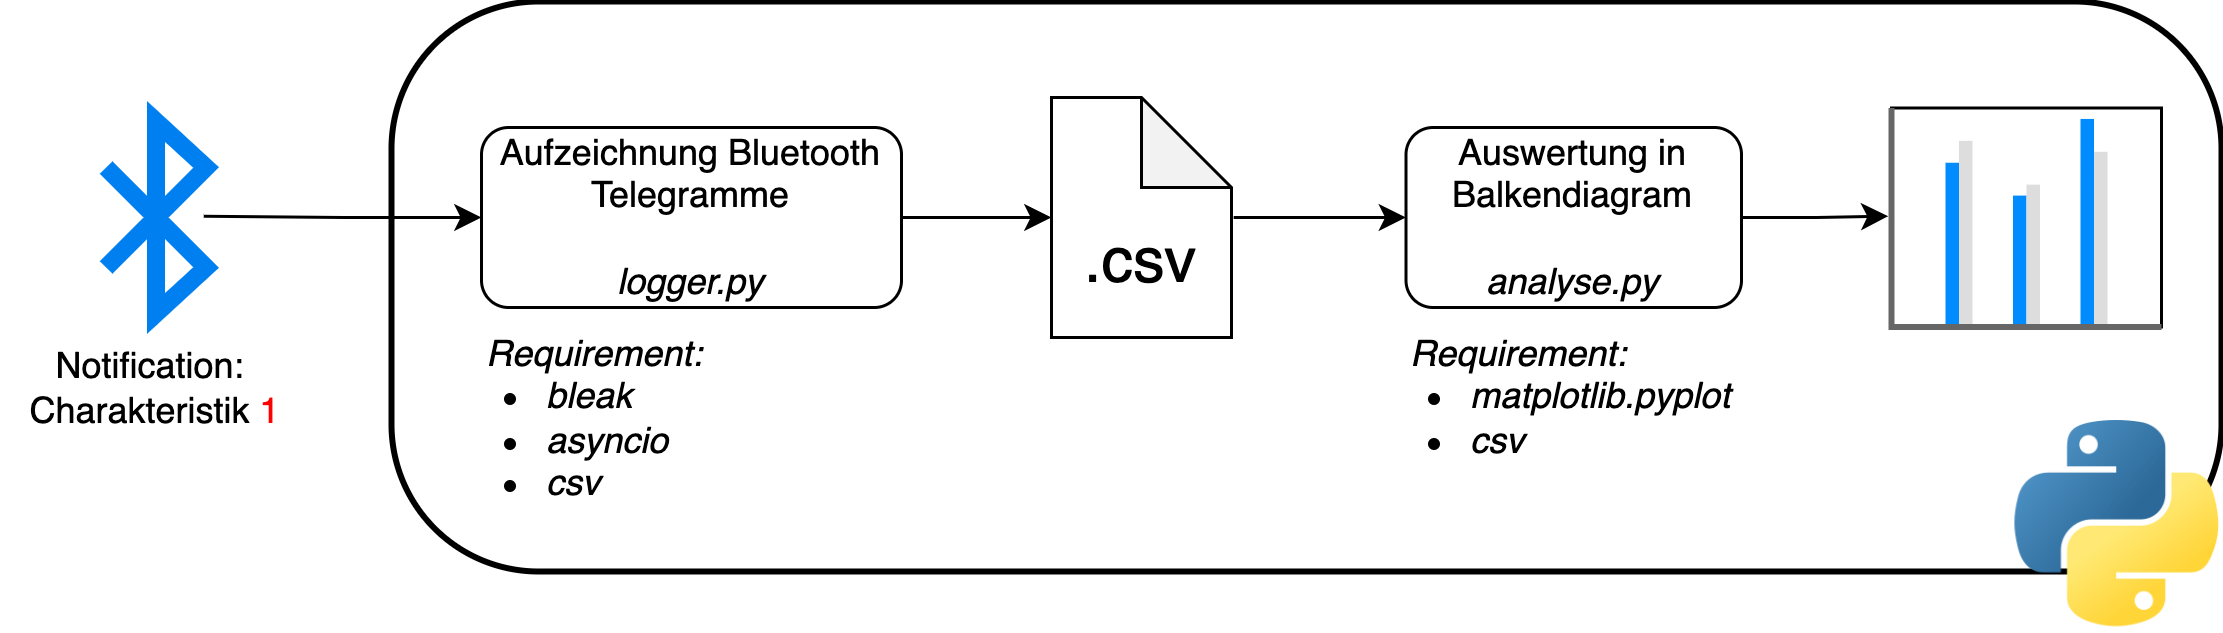
\includegraphics[width=0.9\linewidth]{Figures/Chap3/Testszenarien/Testszenario_Stresstest.png}
    \caption{Testszenario Stresstest}
    \label{fig:TestszStresstest}
\end{figure}

Es werden genau vier unterschiedliche Telegramme erwartet. Diese werden in der Telegrammstruktur von Kapitel \ref{subsub:DataTelegramm} mit dem Payload von Tabelle \ref{tab:frame_data}.

Nun kann gemäss Abbildung \ref{fig:TestszenarioSniffer} das Triggerintervall erhöht werden. In Abbildung \ref{fig:ReineDaten} ist ersichtlich, dass das maximale Intervall 1 ms beträgt. Somit wurden Messungen für 100 ms, 50 ms, 10ms, 1ms durchgeführt.

Die empfangenen Daten werden dann in einem Balkendiagramm dargestellt. Auf der X Achse die Telegramme und auf der Y Achse die Anzahl Telegramme, die empfangen wurden. Erwartet wird, dass vier gleich grosse Balken sichtbar werden.

